\chapter{Installazione e accesso}
\label{Installazione}

\section{Requisiti di sistema}
Di seguito sono riportati i requisiti minimi per utilizzare la skill MegAlexa:

\begin{itemize}
	\item \textbf{Sistema Operativo}: Android 4.4 KitKat API 19;
	\item \textbf{Memoria richiesta}: 50MB;
	\item \textbf{Connessione internet}: richiesta;
	\item \textbf{Dispositivo}: Amazon Echo Dot;
	\item \textbf{Applicazione Alexa installata};
	\item \textbf{Applicazione MegAlexa installata};
	
	
\end{itemize}

\textbf{NOTA BENE:} si consiglia fortemente l'utilizzo di un dispositivo Amazon Echo per un'esperienza migliore. Se non si è in possesso di tale dispositivo c'è la possibilità di acquistarne recandosi nel sito di \href{https://www.amazon.it}{Amazon}.

\section{Installazione applicazione}
Scaricare e installare l'app dal Google \href{https://play.google.com/store/apps?hl=it}{Play Store} sul proprio dispositivo.
\newpage
\section{Avvio applicazione}

Avviare l'applicazione ed effettuare il login con il proprio account Amazon cliccando sul tasto "Login with Amazon".

\begin{figure}[!ht]
	\centering
	\fbox{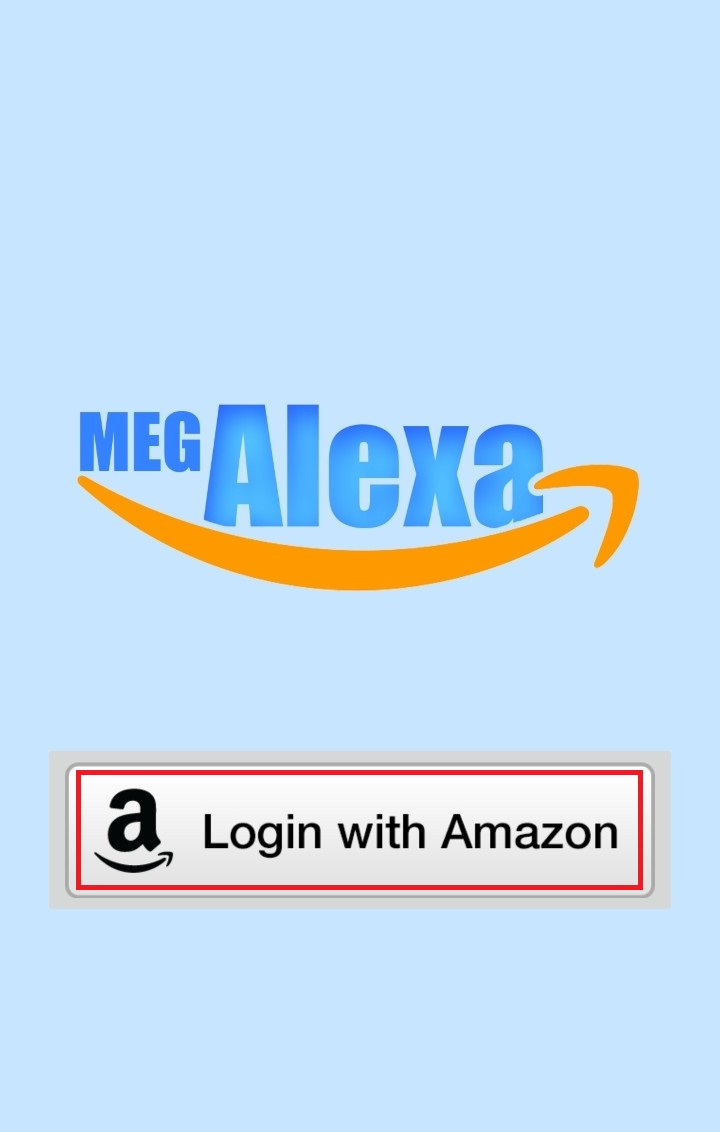
\includegraphics[scale=0.2]{images/Login.jpg}}
	\caption{Pagina iniziale app}
\end{figure}

\subsection{Login con account Amazon}

\begin{enumerate}
\item Se non si possiede un account Amazon cliccare sul tasto "Crea un nuovo account Amazon" e seguire la procedura guidata per creare un nuovo account.
\item Se si possiede un account Amazon:
\begin{enumerate}
	\item Inserire le credenziali del proprio account Amazon;
	\item Cliccare su "Accedi" per effettuare il login.
\end{enumerate}
\begin{figure}[!ht]
	\centering
	\fbox{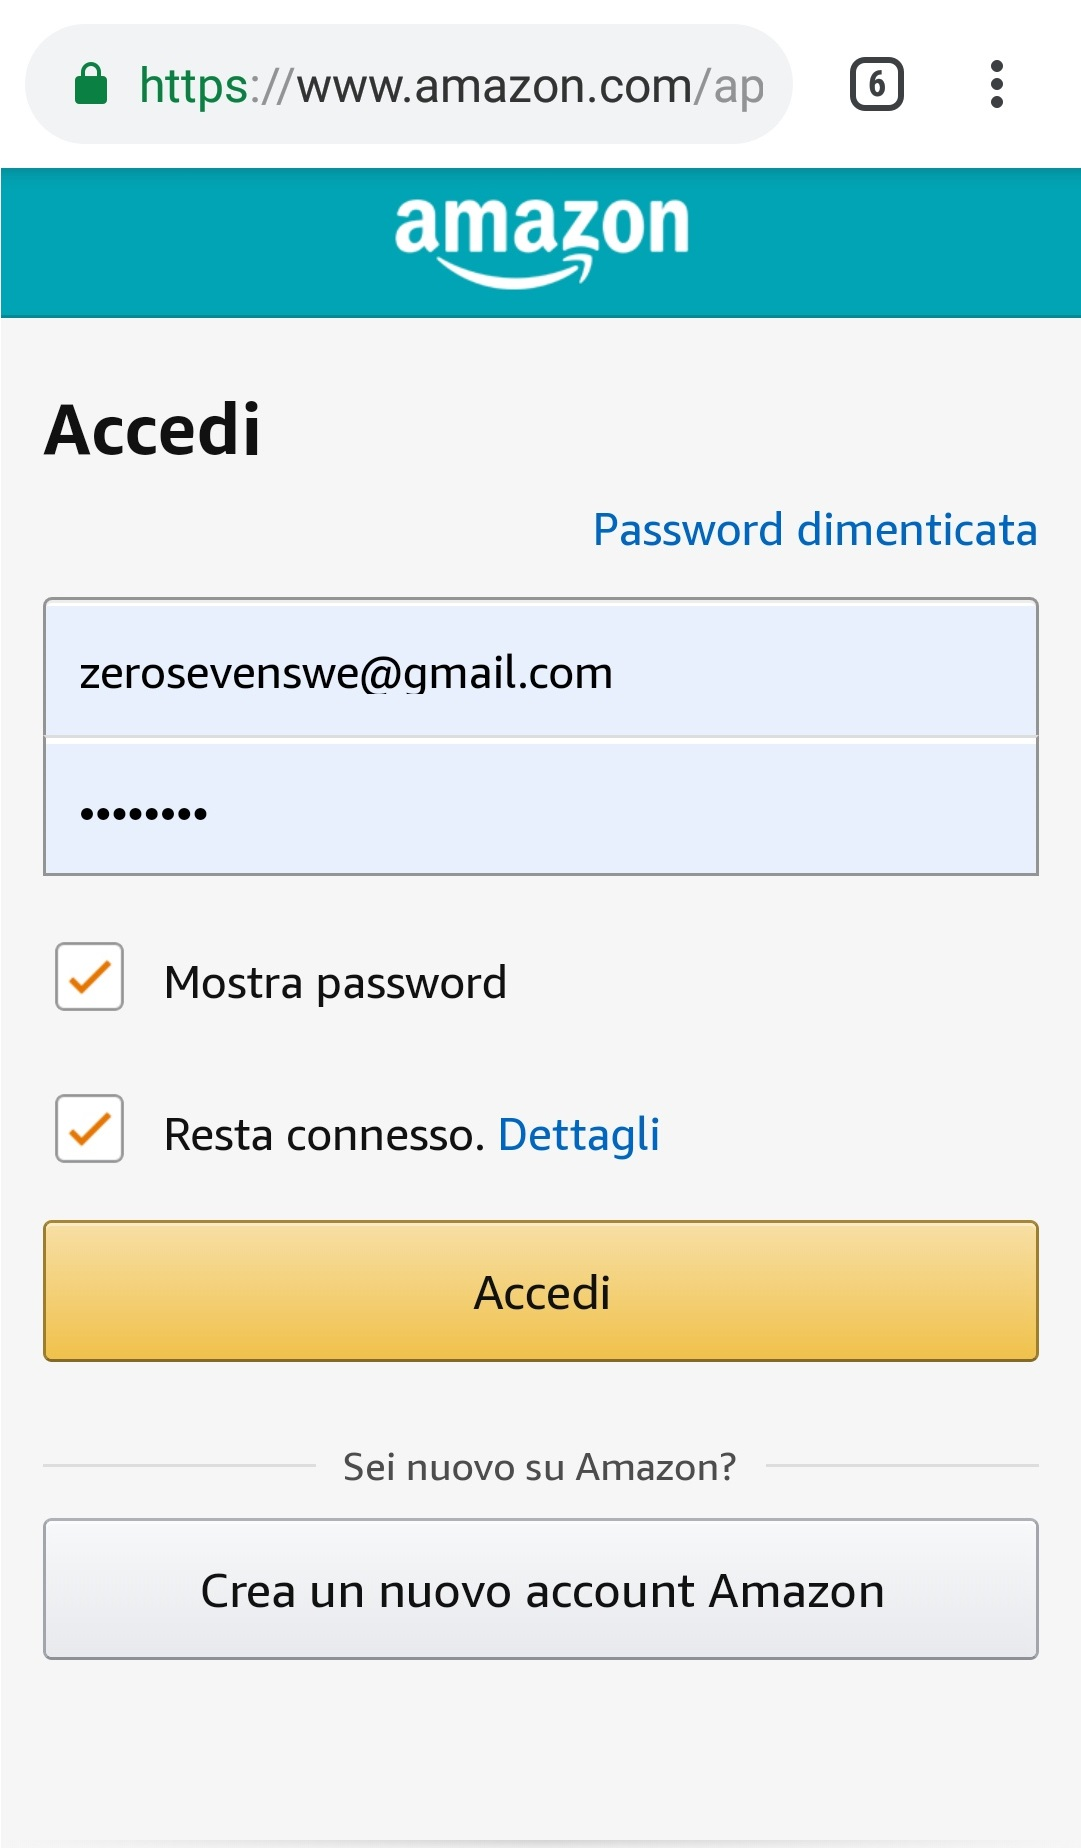
\includegraphics[scale=0.2]{images/Autentication.jpg}}
	\caption{Login ad Amazon}
\end{figure}

\end{enumerate}
\newpage
\subsection{Logout}

\begin{comment}
\begin{figure}[!ht]
	\centering
	\fbox{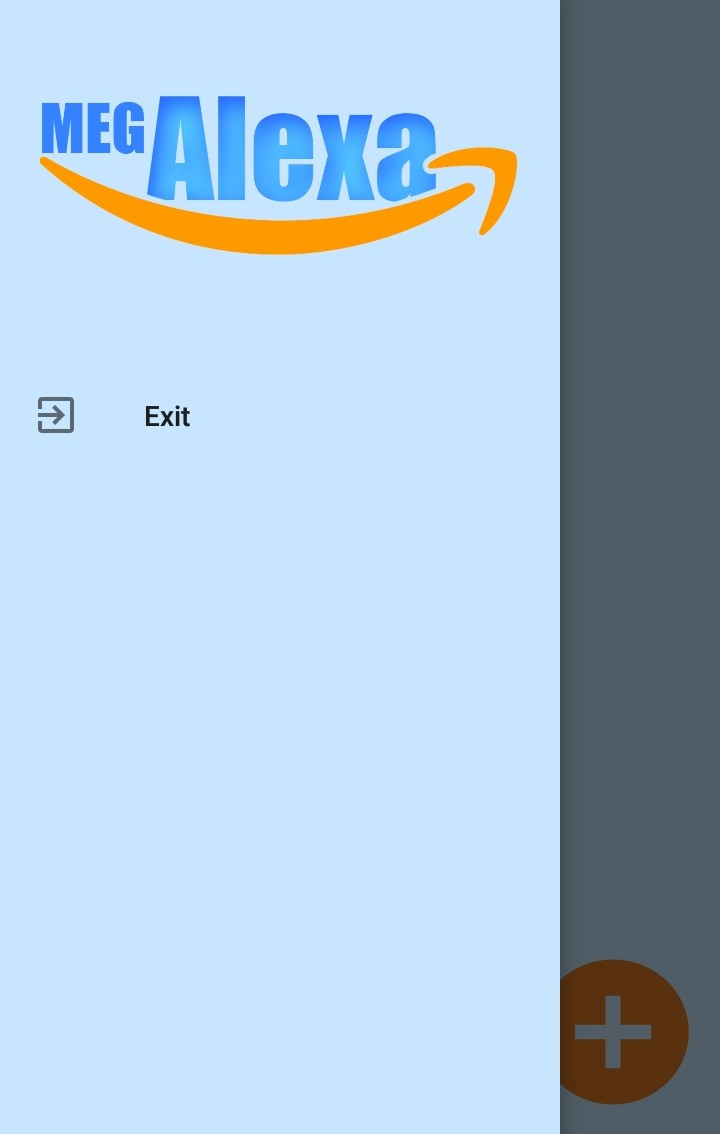
\includegraphics[scale=0.2]{images/Logout.jpg}}
	\caption{Logout}
\end{figure}
\end{comment}

